\documentclass[10pt,a4paper]{report}
\usepackage[english]{babel}
\usepackage{amsmath}
\usepackage{graphicx}
\usepackage{lmodern}
\usepackage[font=small,format=plain,labelfont=bf,up,textfont=it,up]{caption}
\usepackage[nottoc]{tocbibind}
\usepackage{url}
\usepackage{courier}
\usepackage[T1]{fontenc}
\usepackage[titles]{tocloft}
\usepackage{subfig}

\setcounter{secnumdepth}{5}
\setlength{\parindent}{0in}

\renewcommand{\topfraction}{0.85}
\renewcommand{\textfraction}{0.1}
\renewcommand{\floatpagefraction}{0.75}

\makeatletter
\newcommand\ackname{Acknowledgements}
\if@titlepage
  \newenvironment{acknowledgements}{
      \titlepage
      \null\vfil
      \@beginparpenalty\@lowpenalty
      \begin{center}%
        \bfseries \ackname
        \@endparpenalty\@M
      \end{center}}%
     {\par\vfil\null\endtitlepage}
\else
  \newenvironment{acknowledgements}{
      \if@twocolumn
        \section*{\abstractname}
      \else
        \small
        \begin{center}
          {\bfseries \ackname\vspace{-.5em}\vspace{\z@}}
        \end{center}
        \quotation
      \fi}
      {\if@twocolumn\else\endquotation\fi}
\fi
\makeatother

\title{CuEira, gene-enviroment interaction analysis on GPU}
\author{Daniel Berglund}
\date{April 2014}

\begin{document}
\maketitle
\thispagestyle{empty}

\clearpage
\thispagestyle{empty}
\selectlanguage{english}
\begin{abstract}
Abstract in english
\end{abstract}

\clearpage
\thispagestyle{empty}
\selectlanguage{english}
\begin{abstract}
Abstract på svenska
\end{abstract}

\clearpage
\thispagestyle{empty}
\begin{acknowledgements}
Asdf
\end{acknowledgements}

\clearpage
\tableofcontents
\thispagestyle{empty}

\clearpage
\setcounter{page}{1}
\chapter{Introduction}

\section{Genome-wide association studies}
Within Epidemiology genome-wide association studies(GWAS) are a type of study to search for associations between genetic markers and diseases. Classically GWAS does not consider interactions between the genetic markers themselves or with environmental factors. Investigating gene-gene interactions recently has become more common\cite{cordell_detect_review}, however gene-environment interactions are still an uncommon focus in studies\cite{gene_enviroment_2013}. Interactions between genes and environmental factors are considered to be important for complex diseases such as cancer and autoimmune diseases.\cite{cordell_detect_review, gene_enviroment_2013, geira, ra_smoking}\\
\\
GWAS are usually either cohort or case-control. In cohort studies a healthy sample of a population is being followed and over time some individuals will developed the disease of interest. In case-control studies two groups are compared to find risk factors. One group consists of individuals with the disease and the other of individuals that are similar to the cases but who do not have the disease.\cite{rothman1998modern,mann_observational}\\
\\
The genetic markers are commonly single-nucleotide polymorphisms(SNPs). SNPs are variations in the genome where a single nucleotide is different between individuals in a population\cite{fareed_snp}. Environmental factors can be various things such as smoking, physical activity and so on. The amount of data to handle usually consists of thousands individuals and hundred thousands or millions of SNPs. Due to the high number of SNPs few algorithms are capable to investigate more than second order interaction in a reasonable time. There are some algorithms that can handle higher interaction orders however these have drawbacks\cite{gwis,high_order_2012,fast_high_order_cluster}.

\section{GEIRA and JEIRA}
\emph{GEIRA} is a tool for analysing gene-gene and gene-environment interaction. It uses logistic regression and causal interaction\cite{geira}. \emph{JEIRA} is a parallelized implementation of the environmental interaction analysis in GEIRA. However it can only be run on one node.

%TODO something about GEISA

\section{Defining Interaction}
There are several ways to define interaction. The overall goal is usually to find if \emph{biological} interactions are present. \emph{Biological} interaction is when the factors co-operate through a physiological or biological mechanism and causes the effect, eg. disease. This information can be used to explain the mechanisms involved in causing the disease and possibly help to find cures for them. However biological interaction is not well defined and thus it is not possible to calculate it directly from data.\cite{rothman1998modern,rothman2002intro_epidemiology}\\
\\
\emph{Statistical} interaction on the other hand is well defined. However it is scale dependent, ie. interactions can appear and disappear based on transformations of the data. Statistical interaction also depends on the used model. The common way to define statistical interaction is to consider the presence of a product term between the variables in the statistical model, this is referred to as \emph{multiplicative} interaction. For instance for a linear model
\begin{equation}
f(x,y)=ax+by+cxy+d
\end{equation}
c is the product term that represents multiplicative interaction between variables x and y. Statistical interaction is often referred to as just interaction which can make it a bit confusing.\cite{geira,rothman1998modern}\\
\\
It can also be defined as the divergence from additive effects on a logarithmic scale, e.g.
\begin{equation}
OR_{both\:factors\:present}>OR_{first\:factor\:present}+OR_{second\:factor\:present}-1
\end{equation}
It is called additive interaction. It implies biological interaction as defined by Rothman, which is sometimes called \emph{causual interdependence} or \emph{causal interaction}.\cite{rothman1998modern}

\clearpage
\chapter{Background}
%TODO

Most of the conducted research on interactions in GWAS has been focused on gene-gene interactions. Few studies and tools have been investigating gene-environment interactions.

Both CPU clusters\cite{biforce} and GPUs\cite{gwis,gboost,gmdr_gpu,cuda_lr,genie_2012,plink_gpu} have been used for GWAS. GPUs have been a popular choice since most of the methods for searching for interaction are good on GPUs because each combination can usually be considered independently from the others. More about this in section \ref{gpu_gwas}

%Bla bla lite om outline

\section{Mathematical Background}
There are a lot of algorithms and programs proposed for searching for interaction, most have focused on gene-gene interaction as already mentioned. They can be roughly classified into four categories, exhaustive, stochastic, machine learning/data mining and stepwise\cite{fast_high_order_cluster}\\
\\
SNPs are commonly binary variables with either dominant or recessive models. Dominant is when a person only has to have one allele affected to get the trait. Recessive is when both alleles have to be the cause. The case where the risk is present is coded as 1 and absence is coded as 0. Co-dominant model can also be used and in that case when both alleles have the risk factor is coded as 2, when only one is present is coded as 1 and absence is 0 as before. That SNPs can be viewed as binary is an advantage that is almost always used when searching for gene-gene interactions.\\
\\
Environmental factors can be of any type\cite{gene_enviroment_2013}. Gene-gene interaction tools can sometimes be used to find gene-environment interaction, however they usually require the variable to be binary or have other problems since they weren't designed for environmental interaction.\cite{gene_enviroment_2013}\\
\\
\emph{Exhaustive search} is the most direct approach, it compares all combinations of the SNPs in the data. Exhaustive search methods will not miss a signficant combination because it didn't considere it however it also means that they can bee slow. Multifactor-Dimensionality Reduction(MDR)\cite{mdr_2001} and BOOST\cite{boost_gene_gene} are two examples of this type of algorithm.\\
\\
\emph{Stochastic} methods uses random sampling to ``walk'' through the data. BEAM\cite{beam_2007} is one example and it uses Markov Chain Monte Carlo(MCMC) method.\\
\\
\emph{Data Mining} and \emph{Machine Learning} are methods that learn from data and tries to generalize it. MDR\cite{mdr_2001} is a type of data mining method and is among the most common methods used in GWAS. See section \ref{data_machine_learning} for more details.\\
\\
\emph{Stepwise} methods uses a filtering stage and a search stage. At the filtering stage uninteresting combinations are filtered out by using some exhaustive method. The other SNPs are the examined more carefully in the search stage. BOOST\cite{boost_gene_gene} is an example which uses clever data structures and a likelihood ratio test to filter the data before applying log-linear models.

\subsection{Confounders and Covariates}
\emph{Confounding} is one of the central issues in the design of epidemiological studies. It is when the effect of the exposure is mixed with the effect of another variable. So if we do not measure the second variable the first effect would be estimated as stronger than it really is. The second variable is then a \emph{confounder}. Several methods in epidemiology are about avoiding or adjusting for confounding. Sometimes these variables needs to be incorporated into the models. \emph{Covariates} are possible confounders or other variables that one wants to adjust for in the model. Sometimes covariates are called \emph{control variables}.\cite{rothman2002intro_epidemiology,rothman1998modern}

\begin{figure}[h]
    \centering
    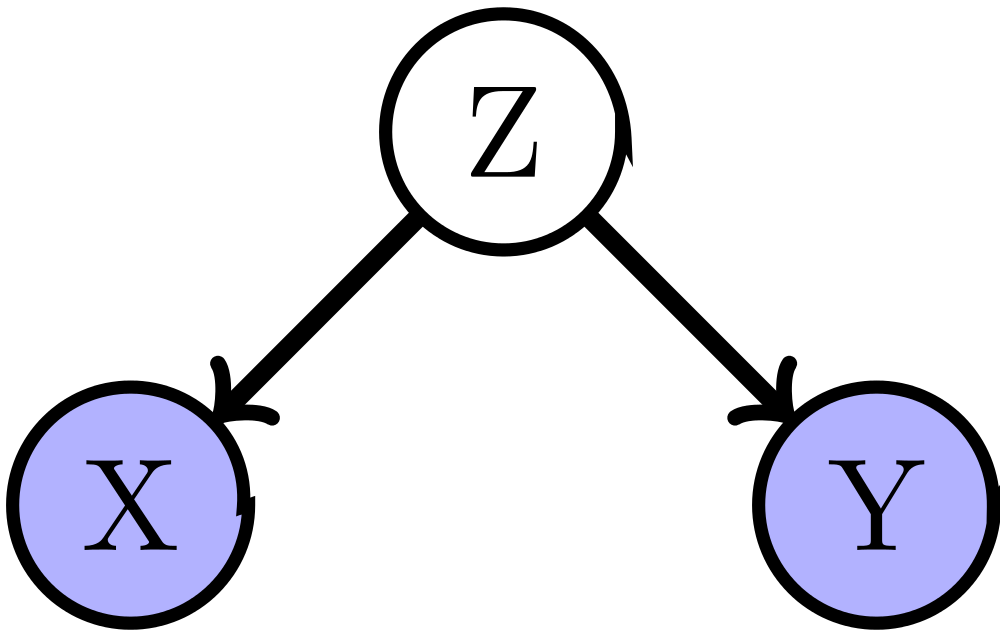
\includegraphics[width=5cm]{Simple_Confounding_Case.png}
    \caption{Illustration of a simple case of confounding. If we do not observe Z we might falesly find an association between X and Y. Wikipedia Commons}
    \label{fig:confunding}
\end{figure}

\subsection{The Multiple Testing Problem}
It is not uncommon to test a lot of hypothesis on the same data and in the case of GWAS it can be billions of tests. If one continues to test one should eventually find something that is significant. Also it is important to remember that the standard p-value of 5\% means that we expect to find 1 in 20 false positives under the assumption that the null hypothesis is true. The problem arises from the fact that the hypothesis tests are dependent on each other since they use parts of the same data. This is the multiple testing problem and if it is not corrected for one might find a lot of false positives.\cite{bonferroni_multiple}\\
\\
Bonferroni correction is the simplest and viewed as the most conservative way to correct for this problem. It simply divides the p-value threshold that a test passes by the number of hypothesis. However the number of hypothesis made is not always clear. With a two-stage analysis, is the number of hypothesis the number of tests done in both stages combined, the number made in the first stage or the second stage?\cite{bonferroni_multiple}

\subsection{Contingency Tables}
A contingency table is a matrix used to describe categorical data. Each cell contains the frequency of occurrences with a specific combination of variables. Table \ref{table:contingency_table} is an example of an 2 x 3 table. From this table we can for instance see that 171 persons that got the placebo had a nonfatal attack. Contingency tables are the basis for various statistical tests to model the data. Contingency tables can be used directly for tests like $chi^2$.\cite{agresti_categorical}

\begin{table}[h]
\begin{tabular}{ l c c c }
  \hline
  & Fatal Attack & Nonfatal Attack & No Attack\\
  \hline
  Placebo & 18 & 171 & 10 845 \\
  Aspirin & 5 & 99 & 10 933 \\
  \hline  
\end{tabular}
\caption{Contingency table describing the outcome of a medical study, from \cite{agresti_categorical}}
\label{table:contingency_table}
\end{table}

\subsection{Logisitic Regression}
One way to model the contigency tables is by using logistic regression. Logistic regression is a type of linear regression model for classification that models a latent probability for the outcomes. The outcomes are commonly considred binary, however it can be extended to multiple outcomes. In this work we will only consider them as binary. Logistic regression transforms the probability by using the \emph{logit} transformation. The logit transformation with probability \emph{p} is 

\begin{equation}
log(\frac{p}{1-p})
\end{equation}

%picture of logit transformation graph

The probability with a set of predictor variables \emph{X} is $\pi(X)=P(Y=1)$. The linear regression model with n predictors $X=(x_1,x_2,....,x_n)$ and by using the logit transformation is then
\begin{equation}
logit[\pi(X)]=\alpha+\beta_1 x_1+\beta_2 x_2+...+\beta_n x_n
\end{equation}

If move the logit to the right side we get the moddelling of the probability
\begin{equation}
\pi(X)=\frac{exp(\alpha+\beta_1 x_1+\beta_2 x_2+...+\beta_n x_n)}{1+exp(\alpha+\beta_1 x_1+\beta_2 x_2+...+\beta_n x_n}
\end{equation}

Finding the coefficents are done in a similar way as other linear regression models since they all are generalized linear models. It's done using  maximum likelihood(ML), often via Newtons method.

It's an iterattive method which means it is slow compared to non iterative mehtods. Logistic regression as most other methods for interaction assumes independecne between the variables.

\subsubsection{Statistic Measures}
There are various statistical measures of interest that we can calculate from the logistic regression model.\\
\\
Odds ratio(OR) describes the change in odds between different levels of exposure.

The odds is ?

In binary case it simplifies to the increased odds when exposed.

An odds ratio of one means the the odds and therefore the odds is the same whetever exposed or not. An odds ratio below one means that the odds of being affected is lower when exposed and if the odds ratio is above one it means that the odds is increased. In the case when the outcome is an disease or similar we call variables with odds ratio below one \emph{protective} and when it is above one it is a \emph{risk factor}.

Relative risk(RR)
\begin{equation}
RR=\frac{p_{event\:when\:exposed}}{p_{event\:when\:not\:exposed}}
\end{equation}

RR can not be esitmaded in case control since it requires the prevalence in whole population which you need cohort studies to find. In case control it is approximate with OR.

Relative  excess risk due to interaction(RERI) is
\begin{equation}
RERI=RR_{11}-RR_{10}-RR_{01}+1
\end{equation}
%cite rothman? chapter 15

Attributable proportion due to interaction(AP)
\begin{equation}
AP=\frac{RERI}{RR_{11}}=\frac{1}{RR_{11}}-\frac{RR_{10}}{RR_{11}}-\frac{RR_{01}}{RR_{11}}+1
\end{equation}

Synergy index(SI)
\begin{equation}
\frac{RR_{11}-1}{RR_{10}+RR_{01}-2}
\end{equation}

SI is simpler to investigate on the log scale
\begin{equation}
ln(SI)=ln(RR_{11}-1)-ln(RR_{10}+RR_{01}-2)
\end{equation}

Lack of interaction shows in the values by
AP=0
SI=1

\subsubsection{Coding the interaction variable}
%TODO
For the interaction

%math stuff for mult

%math stuff for add

However there is a problem when there is multiple categories in both variables. In short it's becase of how OR works and that the categories for LR become rated in increased or decreased order, that is how the categories are labeled matters. Say three locations, code as 1,2,3 or 2,1,3 matters. 

There is two cases, 
one were we don't know any severness or whatever, say locations

second were we do have it, say it's smoking as never, previous and current. current is likely worse than previous worse than never

but if the second one also has levels say it's also of second type as simplest case example here
how do we know which is worst? current smoker or exampel badest
number of possiblitys increases with levels and to examine all means lots of computions and loss of statistical powers

Why occurs due to how OR works

However in our case we know that the gene is binary under dominat or recessive model. So we can just multiply. However means we can't use co-domiant model.

Dummy variables
Stratification

\subsubsection{Recoding}
%TODO ask Henrik about refrences and why etc

\subsection{Data Mining and Machine Learning Approaches}
\label{data_machine_learning}
Approaches based on Data Mining and Machine Learning have been a popular choice for GWAS. Multifactor-Dimensionality Reduction(MDR)\cite{mdr_2001} and Random Forest(RF)\cite{random_forest} are among the most common ones\cite{gene_enviroment_2013,cordell_detect_review}. There are other methods as well such as clustering approaches \cite{fast_high_order_cluster}. Most of them are used for screening the data for possible interactions\cite{gene_enviroment_2013,cordell_detect_review}.\\
\\
Their biggest advantage is that they are usually nonparametric and designed with high dimensional data in mind. However they are prone to overfitting and the usual way to try to prevent that is to use cross validation and sometimes permutation tests. It means that even if the method itself is fast it is repeated so many times that the whole algorithm can be slow in the end.\cite{cordell_detect_review}

\subsubsection{Multifactor-Dimensionality Reduction}
Multifactor-Dimensionality Reduction(MDR) is a method that reduces the number of dimensions by combining several dimensions into one. For GWAS it combines a number of variables from all the variable combinations and its new dimension is then compared against the outcome. If its predictability is high then the variables that were combined are considered to interact with each other. MDR repeates the process on all combinations of variables. It combines the selected n variables by calculating the ratio of cases versus controls for each combination of the possible values of the variables. If the ratio is above a certain threshold all the members of that groups is gets the value 1 for the new dimension, otherwise 0. However due to the cross validation and permutation tests this method can be slow. On the other hand it is still faster than exhaustive search with regression methods.\cite{cordell_detect_review,mdr_2001}\\
\\
An simple example of MDR using exclusive or(XOR). XOR is an logical operator that is true if one and only one of its two variables is true. We have 4 possible combinations and an occurrence for each of them. The combination (1,0) and (0,1) both have one case with outcome 1 so MDR will classify them as 1 in the new variable Z. The other two combinations have outcome 0 so will be classified with Z=0. From here it is easy to make an predictor from Z to the outcome Y by comparining the values.

\begin{table}[h]
\begin{tabular}{ | c | c | c | }
  \hline
  \textbf{Y} & $\mathbf{X_1}$ & $\mathbf{X_2}$ \\
  \hline
  1 & 1 & 0 \\
  \hline 
  1 & 0 & 1 \\
  \hline
  0 & 0 & 0 \\
  \hline
  0 & 1 & 1 \\
  \hline
\end{tabular}
\caption{XOR table with outcome $\mathbf{Y}$ and variables $\mathbf{X_1}$ and $\mathbf{X_2}$.}
\label{table:xor_table}
\end{table}
\begin{table}[h]
\begin{tabular}{ | c | c | }
  \hline
  \textbf{Y} & \textbf{Z} \\
  \hline
  1 & 1 \\
  \hline
  1 & 1 \\
  \hline
  0 & 0 \\
  \hline
  0 & 0 \\
  \hline
\end{tabular}
\caption{XOR table with $\mathbf{X_1}$ and $\mathbf{X_2}$ combined into $\mathbf{Z}$ using MDR.}
\label{table:xor_mdr_table}
\end{table}

MDR can been used for gene-environment interaction but requires modifications since MDR can only handle binary variables. There are extensions that can use continues variables, however these are regression based so these will be slower than regular MDR.\cite{gene_enviroment_2013}

\subsubsection{Random Forest}
Random Forest(RF) is an ensemble learning method. Ensemble methods combine multiple models to improve performance. RF takes randomized samples of the data and builds decision trees on each of them. These trees are then combined to form the classifier. Usually hundreds or thousands of trees are used depending on the problem\cite{random_forest}. One of the most popular variants of Random Forest for GWAS is Random Jungle\cite{random_jungle}.\\
\\
It has been shown in high dimensional data that RF tends to only rank interacting factors high if they have strong marginal effects\cite{winham_rf_2012}. Also the ranking of the variables does not indicate which factor it is interacting with either since it is based on the joint distributions\cite{gene_enviroment_2013}. How to incorporate the environmental factors in RF is also not obvious and using variables with very different scales can bias RFs results\cite{gene_enviroment_2013}.

Decision tree figure here

\clearpage
\section{Computer Architecture}
Most computers today have a multi-core architecture
means several processors share the main memory and other resources. they can cooperate on the same problem but it they are coordinated on a case by case basis since each algorithm requires different sharing.

Von Neumann architecture
It was first used in EDVAC which was one of the first stored program computers\cite{von1993first}. Stored program computers uses electronic memory to store the program instructions\cite{computer_arch_2003}.

\begin{figure}[h]
    \centering
    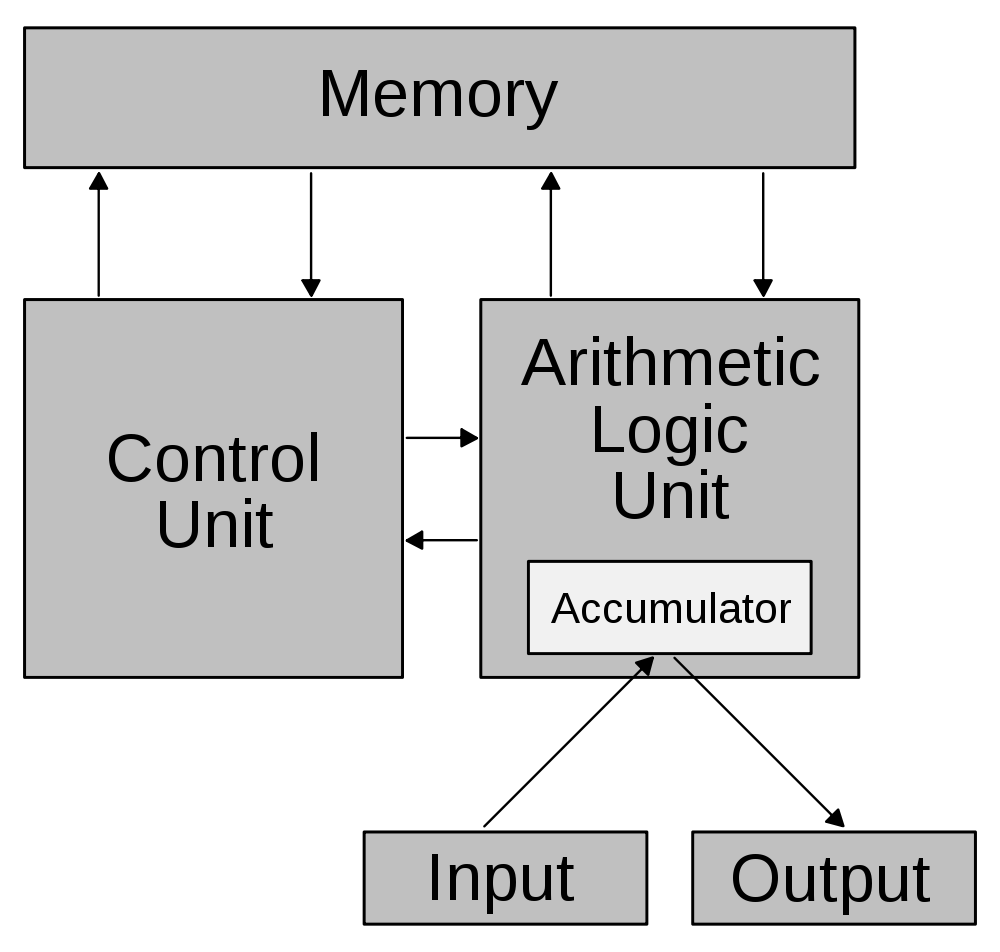
\includegraphics[width=7cm]{Von_Neumann_architecture.png}
    \caption{Schematic of the Von Neumann architecture. Wikipedia Commons}
    \label{fig:VonNeumann}
\end{figure}

some text here about von neaumann architecture

For HPC it is easiest to think about the architecture as three main parts, data storage, processor and the memory. More text here\cite{intro_hpc}

\subsection{CPU}
Central processing unit(CPU) is \cite{introduction_hpc_hager}

Until 1996 there was computers with just a single core CPU on top 500\cite{TOP500}. Since about 2005 most desktop computers CPU has several cores which has increased the need for parallelization. The cores themselves aren't getting faster, the CPUs have more cores.

%schematic here

As you can see most of it is not used for calculations. A large part of the area is used for optimizations and caching. We will talk about caching in the next section. CPUs have various optimizations too improve their performance.

branch prediction

\subsection{Caching and Other Optimization}
%TODO
The CPU optimzation that is most important to know for programmers is caching because it affect the way the code has to be written and the diffrence between using it correctly and not is huge.

%aliasing
It happens when two pointers point to the same place in memory and the code does operations on them at the same place. This means that operations that look like they can be done in any order actually can't and thus prevents the compiler to make optimizations. The problem is that the compiler has to take this in to account for all pointers even if no aliasing occurs because it might happen.

\cite{drepper2007cpumemory}

\subsection{Concurrency and Threads}
%TODO
concurrency what is it

doing multiple things and the same time, instead of \emph{sequential}

dinning philosphers

in computer science, instructions seperated in threads

SIMD

MIMD

\cite{introduction_hpc_hager}

\subsection{Accelerators, GPU and Xeon Phi}
Graphics processing unit(GPU) have become more popular for general computing the last 10 years.

\begin{figure}[h]
    \centering
    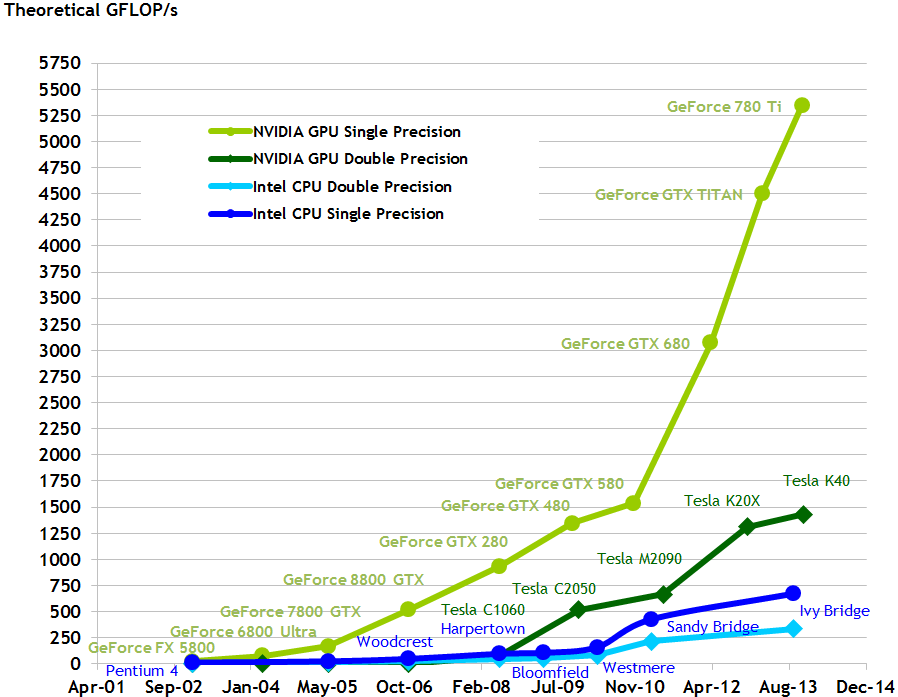
\includegraphics[width=11cm]{floating-point-operations-per-second.png}
    \caption{Bla bla \cite{cuda}}
    \label{fig:gpu_vs_cpu}
\end{figure}

%structure of gpu

'dummer' threads than CPU, more area for calculations

Xeon Phi, intel mic
mimd
knights landing, interesting new development from intel.
however usually but not always require memory copy
still need vectorisation and other stuff
you end up with similar problems as gpu, though probably easier to use

structure of mic

\subsection{Which program for GPU and which for CPU?}
\label{gpu_gwas}
As with a lot of things it depends on the algorithm to implement etc.

If you have lots of legacy code then then you might need to rewrite a lot. However by using a profiler the parts that take up the most time can be found and moved to the GPU. However that migh be hard if the program isn't properly structured. No legacy code can also be a good thing. Old code might not be written with modern standards or use new nifty features and therefore lose speed.

Xeon Phi is an alternative, simpler but can still be tricky and require memory copy.

GPUs loses more when going from single precision to double than CPUs. Peak performance on tesla-kepler cards for single precision is around 4 Tflops while double precision is around 1.4 Tflops. \cite{nvtesla}\\ ref the table, single is much faster than double

In short GPUs excel at linear algebra but Intel MIC is probably a good alternative for it to.

GPUs are good for interaction algorithms since most approaches are embarrassingly parallel since they consider each combination independently from the others. They also often perform a lot of linear algebra. Several studies got high gains from implementing their programs on GPU, however their CPU versions weren't parallelized so it is likely that the gains would have been less compared to an optimized and parallelized CPU version.\cite{gwis,gboost,gmdr_gpu,cuda_lr,genie_2012,plink_gpu} However one study made a CPU cluster version and a GPU version of an algorithm that uses $chi^2$ tests, they found that 16 CPU nodes had the same performance as a single GTX 280 card\cite{jiang_accelerating}.

\subsection{Clusters}
Clusters are collections of computers that can work together in several ways and are so tightly connected that they can usually be viewed as a single system. They communciate over a shared network but have separate memory and processors. Storage is usually shared. A computer in a cluster is called a \emph{node}. \cite{intro_hpc, kirk2012programming}

various programming models, shared memory and so on
%shared memory, cache coherrency and stuff

mpi is commonly used for clusters\cite{kirk2012programming}

top 500\cite{TOP500}

Few clusters used GPUs before 2009 but now mix of GPUs and cpu are common among the top clusters. It was driven largely by demand for power saving while still giving high performance. The GPUs can do the heavy computation while other parts are used on CPU. Most of these clusters are highly ranked in Green 500. \cite{kirk2012programming}
%Something about Intel MIC

Flops is not everything, bad performance compare to theoretical maximum
Stuck in network, hard drives, etc. Latency
Very few programs scale to the fastest clusters, peta scale.

Tianhe 2 is current top. Theoretical performance 54.9 PetaFlops.\cite{TOP500}
Max achived with LinPack 33 PetaFlops
60\% efficiency

Picture of Tianhe-2 here

\subsection{CUDA programming model}
Cuda function calls are done by using kernels
divided into blocks

These blocks can be executed in any order so depending on the number of streaming multiprocessors(SM) they get executed differently

\begin{figure}[h]
    \centering
    \includegraphics[width=10cm]{automatic-scalability.png}
    \caption{Text abou blocks. Need to make a black white verison}
    \label{fig:blocks_scaling}
\end{figure}

Kernels are declared by using the \_\_global\_\_ specifier 
setting stuff for the call to the kernel by using <<<...>>>

%simple kernel example here

The blocks are organized in one, two or three dimensional \emph{grid}. These can be accesed in a kernel.
each block also share some memory, see efficient cuda part or the cuda programming guide for the details.

\begin{figure}[h]
    \centering
    \includegraphics[width=10cm]{grid_2d.png}
    \caption{2d grid of blocks}
    \label{fig:grid_2d}
\end{figure}

The streaming multiprocessors can execute hundreds of threads concurrently, it uses \emph{SIMT}(Single-Instruction, Multiple-Thread).
It executes on groups of 32 threads called warps
when an SM gets a number of blocks they are split into warps that are assigned to warp schedulers
each warp scheduler gives one instruction to the whole warp so full efficiency is achieved when all 32 threads do the same instruction. if there is any divergence it has to disable unrelated threads, so divergence is costly. different warps can diverge without problem

since the GPUs memory is physically on a different device, the \emph{host} and \emph{device} have separate memory spaces. They are referred to as \emph{host memory} and \emph{device memory}. Because it is separate data has to be transferred to the device and this is done by explicit calls to transfer sections of the memory.

%shared memory and other memory types, here or in efficient cuda?

The kernel calls can be made on a stream. By default a kernel is executed on the null stream. The easiest way to think of the stream is as queue, the kernels on a stream will be executed in the order they are made but different kernels from different streams can be executed in any order and if there are resouraces enough at the same time. In this way it is possible to execute up to 32 concurrent kernels depending on GPU.

Streams are important for asynchronous transfers. These transfers are executed on a stream and just as kernels gets executed after the previous kernels on the same stream is done. And as with the kernels the transfer on one stream can happen . This however depends on the number of copy engies and kernel engines. Some older GPUs have one copy engine and one kernel engine. Newer ones have one copy engine for device to host and one for host to device. This can affect how the calls should be ordered and using the wrong one can make the performance worse than without using asynchronous transfers.

%example from the fortran stuff with graphs and such

CUBLAS is provides blas functions for cuda.
can also be run concurrently with streams

%single vs double precision

As already mentioned different architectures and even different GPUs differ how they work. Make sure to lookup the different specifics and read the guides for the relevant architecture. NVIDIA uses something called computational capability. It ranges from 1.0, 2.0, 3.0, 3.5 and 5.0. The higher the number the more functions. 1.0 and 2.0 lack some of the things described here.

\cite{cuda}

\subsubsection{Efficient CUDA}
One of the main criticism against GPUs for general computing purposes is that it is hard to get good performance because it requires good knowledge about details of the GPU architecture, especially the memory architecture. Here are somethings that needs to be considered when writing GPU programs.\cite{plink_gpu, cuda, cuda_best_practice}
\\
\begin{description}
  \item[Maximize parallelism] \hfill \\
  Structure the program and the algorithm in such a way that it is as parallel as possible and overlap the serial parts on CPU with calculations on the GPU.\cite{plink_gpu, cuda}
  \item[Minimize transfers between host and device] \hfill \\
  Moving data between host and device is expensive and should be avoided if possible. It can be better to run serial parts on the GPU rather than moving the data to the host to do the calculation on the CPU. The bandwidth between host and device is one of the large performance bottlenecks. This can be a problem when the data is to large to fit in the relatively small GPU dram.\cite{cuda, cuda_best_practice}
  \item[Find the optimal number of blocks and threads] \hfill \\
  There are a lot of things affected by the number of blocks and threads so they should be considered carefully. It is a good idea to parameterize them so that they can be changed for future hardware and varied for optimization. NVIDIA has an occupancy calculator which can be helpful in determining the optimal numbers, however high occupancy does not mean high performance.\cite{cuda, cuda_best_practice}\\
  \\
  The number of blocks should be larger than the number of multiprocessors so that all multiprocessors have at least one block to execute. Having two blocks or more per multiprocessor can be good so that there are blocks that aren't waiting for a \_\_syncthreads() that can be executed. However this is not always possible due to shared memory usage and similar.\cite{cuda_best_practice}\\
  \\  
  The number of threads per block should be a multiplier of 32 but minimum 64. It's also important to remember that multiple concurrent blocks can reside on the same multiprocessor. Too large number of threads in a block and parts of the multiprocessor might be idle since there aren't a block small enough to use those threads. Between 128 and 256 threads is a good place to start.\cite{cuda_best_practice}
  \item[Streams, concurrent kernels and asynchronous transfers] \hfill \\
  By using streams it is possible to overlap memory transfers with calculations. This means that the data for the next batch can be transfered while the current batch is calculated and when it is done it can start calculating on the next batch directly after the current one is done. This can hide the time for transfers completely in some situations. However it requires the memory on the host to be pinned. Pinning too much memory can reduce performance of the host.\cite{cuda}\\
  \\
  Operations on a stream is guaranteed to be done in the order they are made however calls on different streams can be executed in any order. Some GPUs allow kernels from different streams to be executed concurrently which can be a big boost if the kernels small enough to fit on the multiprocessors at the same time. Up to 16 or 32 kernels, depending on GPU, can be executed at the same time.\\
  \\
  However it requires tweaking of the code that is specific to the GPUs architecture. For instance FERMI architecture only has one queue for the kernels which means that we can get false dependency between kernels. If we have a batch of small kernels and issue them on stream one first and then stream two all the kernels in stream two will be stuck in the queue waiting for the kernels in stream one to finish, this is because the second kernel on stream one has to wait for the first kernel since they are in the same stream. The second kernel then blocks the queue from moving forward so it will not see the kernels on stream two that could be executed. Kepler GPUs on the other hand has several queues so it won't be a problem on those GPUs. It's the same with asynchronous transfers, some GPUs only have one copy engine while others have one engine for device to host and one for host to device.\cite{cuda, overlap_transfers_cuda, kepler_tuning_guide}
  \item[Use the correct memory on the GPU] \hfill \\
  Correct use of caches and memory is important for CPU\cite{drepper2007cpumemory}. It's also important on GPUs but it gets more complicated since the caches are smaller and there are several types of memory.
    \begin{itemize}
    \item Register memory is located on the multiprocessor and usually costs zero cycles to access. The multiprocessor splits the available registers over its threads so if there are a lot of threads that uses a lot of variables not all of them will fit in the register. This is why a program sometimes can be faster with lower occupancy.
    \item Global memory is the main memory of the GPU and is accessible from all threads and blocks. However it is relatively slow to access.
    \item Shared memory is shared inside a block and is faster than global memory. However it is limited in size.
    \item Constant memory is small however its cached so it is fast to access. It's read only and best used for small amount of variables that all threads access.
    \item Local memory is tied to the threads scope, but it is still resides off-chip so it has the same access time as global memory.
    \item Texture memory is read only and can be faster to access than global memory in some situations. This was more important in older GPUs when global memory wasn't cached.\cite{plink_gpu, cuda}
    \item Read-only cache is available on Kepler GPUs and uses the same cache as the texture memory. The data as to be read only each multiprocessor can have up to 48kb of space depending on GPU.\cite{kepler_tuning_guide}
  \end{itemize}
  \item[Avoid divergence] \hfill \\
  Each thread in a warp executes the same instruction at the same time so if some of threads diverge the rest will be ideal until they are at the same instruction again. This means it is important to use control structures such as if statements carefully to prevent threads from idling.\cite{cuda, cuda_best_practice}
  \item[Avoid memory bank conflicts when using shared memory] \hfill \\
  Shared memory is divided into equally-sized memory modules called banks that can be accessed at the same time for higher bandwidth. Bank conflicts occur when separate threads access the same bank. On some GPUs it is fine if all threads access the same bank. Bank conflicts are split into as many conflict-free requests as needed.\cite{cuda, cuda_best_practice}
  \item[Use existing libraries] \hfill \\
  Instead of writing everything from scratch it is usually a good idea to use already existing libraries. Especially when performance is important and most task are non trivial on GPUs so using an already optimized library is a good idea. Some of the most popular libraries for CUDA are:
  \begin{itemize}
    \item CUBLAS: BLAS implementation for CUDA\cite{cublas}
    \item CULAtools: BLAS and LAPACK implementation for CUDA for both dense and sparse matrices\cite{culatools}
    \item MAGMA: BLAS and LAPACK implementation among other things that can distribute the work on both CPU and GPU\cite{magma_2010}
    \item Thrust: Template based library that tries to emulate C++ standard library\cite{thrust_gpu}
  \end{itemize}
  \item[Avoid slow instructions] \hfill \\
  There are some instructions that can be slow and should be avoided if possible, for instance type conversion, integer division and modulo. If a function is called with a floating point number that might be used as a double and require a conversion. By putting an f at the end of the number it is told to be single precision float, for instance 0.5f. In some cases it is possible to use bitwise operations instead which is faster.\cite{cuda, cuda_best_practice}
  \item[Restricted pointers can give increased performance] \hfill \\
  Aliasing can be a problem as mentioned earlier. By using the \_\_restrict\_\_ keyword on pointers the compiler can be told that no aliasing will occur, however it is up to the programmer to make sure that is the case or there might be unexpected results. Not using aliasing reduces the number of memory accesses the CPU needs to make. However it increases register pressure so it can have an negative effect on performance.\cite{cuda}
  \item[Use fast math functions if precision isn't needed] \hfill \\
  There are two versions of runtime math functions. The ones of the type funcf() is slower but more accurate than \_funcf(). The option -use\_fast\_math makes the compiler change all the funcf() to \_funcf().\cite{cuda_best_practice}
\end{description}

%TODO
%Some stuff for multi gpu
%They dont share memory but gpu-gpu memory copys are faster if they are connected since it does not involve the cpu

%unrolling is really good, see volkovs stuff, instruction level parallelism
%unrolling also works on CPUs

\clearpage
\subsection{Performance Measures}
An important part in making fast and efficient programs is to know how fast the program is under certain conditions and which parts of the program are slow. For instance the speed could suddenly drop when we start using to many threads, there might be a bottleneck in the network, and so on.\\
\\
There are two ways to measure how long a program takes to execute. Execution time, sometimes called wall clock time, is how long real life time the program took. The other is to measure the number of processor cycles spent. A parallel program will have shorter execution time than it is serial version however it will likely have spent more processor cycles due to overhead from communication and initialization of the threads. We are usually interested in execution time however number of cycles can be useful for comparison of algorithms.\\
\\
speed up is measures how much faster then program is with a certain number of threads compared to the serial version. It's defined as
$$S(p)=\frac{T(1)}{T(p)}$$
Where $T(1)$ is execution time of serial program and $T(p)$ is execution time of parallel program with p threads. Linear speed up is when S(p)=p, it is sometimes called perfect speed up.\\
\\
Efficieny reflects how efficient the program is using p threads. Linear speed has efficency 1. It's defined as
$$E(p)=\frac{S(p)}{p}=\frac{T(1)}{pT(p)}$$
\\
Strong scaling refers to how the program handles a fixed problem size and increased number of processors. An program with strong scaling has linear speed up. Weak scaling refers to the execution time of the program when there is a fixed problem size \emph{per processor} and the number of processors is increased.\cite{cuda_best_practice}\\
\\
It can be a good idea to plot these measures while varying p, this can show when bottlnecks occur. Looking at the measures at node level can also be useful to get an idea of how increased number of nodes and therefore increased communication affects the performance.

\subsubsection{Amdahl's Law and Gustafson's Law}
Amdahl's Law is used to find the expected speed up of a system when parts of is parallelized. Simply it says that as the number of processors increases the parts that aren't parallelized will start taking up more and more of the wall clock time and that the speed up for adding more processors will decrease as more and more processors are added and more time is spent relatively on the non parallelized part. It's closely related to strong scaling.\cite{cuda_best_practice,2010_reevaluating_amdahl}\\
\\
It says that the expected speed up with F fraction of the code parallelized and p threads is 
$$S(p)=\frac{1}{(1-F)+\frac{F}{p}(1-F)}$$
As the number of threads grow towards infinity $S(p)$ converges on $\frac{1}{1-F}$. If we have 90\% of a code parallelized then even with infinite number of threads we won't get a better speed up than ten.\cite{2010_reevaluating_amdahl}

\begin{figure}[h]
    \centering
    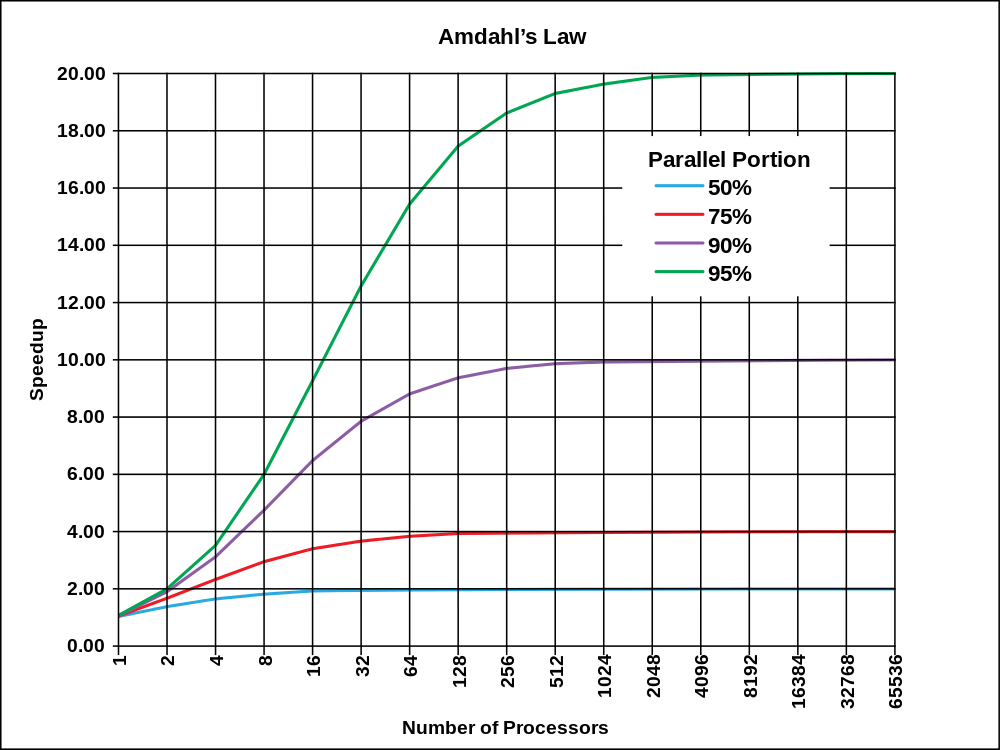
\includegraphics[width=11cm]{AmdahlsLaw.png}
    \caption{Illustration of Amdahls Law. Wikipedia Commons}
    \label{fig:AmdahlsLaw}
\end{figure}

There are limitation to Amdahl's Law since it makes a couple of assumptions.

\begin{itemize}
  \item The number of executing threads remain constant over the course of the program.
  \item The parallel portion has perfect speed up. Often not true due to shared resources,eg caches, memory bandwidth, and shared data.
  \item The parallel portion has infinite scaling, not true due to similar limits as above. More threads will not increase performance after a while or might even decrease it.
  \item There is no overhead for creation and destruction of threads.
  \item The length of the serial portion is independent of the number of threads. Often the serial work is to divided the work to the threads, this work will obviously increase as the number of threads go up. More threads can also lead to more communication overhead.
  \item The serial portion can't be overlapped by the parallel parts. For instance with producer consumer type pattern the consumer could be strictly serial but the time it takes could be overlapped by the parallel producers.
\end{itemize}

This means it is most accurate with programs that are of the fork-join type. Eg serial parts and then matrix operations.\\
\\
Gustafson's Law is closely related to Amdahl's Law and can in some ways be more accurate than Amdahl's Law. Gustafson's Law makes similar assumptions as Amdahl's Law however it also makes two additional statements. It states that problems tends to expand when provided with more computational power, eg increased precision by reducing grid size, high frame rate for graphics. The second is that the parallel portion of the program tends to expand faster than the serial part, eg for matrix multiplication the initialization scales linearly with the matrix size while the multiplication itself scales as $O(n^3)$. The former means that it is closely related to weak scaling. So in a way it says that the execution time remains constant rather than the amount of data. More precise it says that the expected speed up with p threads and F fraction of the code that is parallel is\cite{gustafson1988reevaluating, cuda_best_practice}
$$S(p)=p+(1-F)(1-p)$$

\begin{figure}[h]
    \centering
    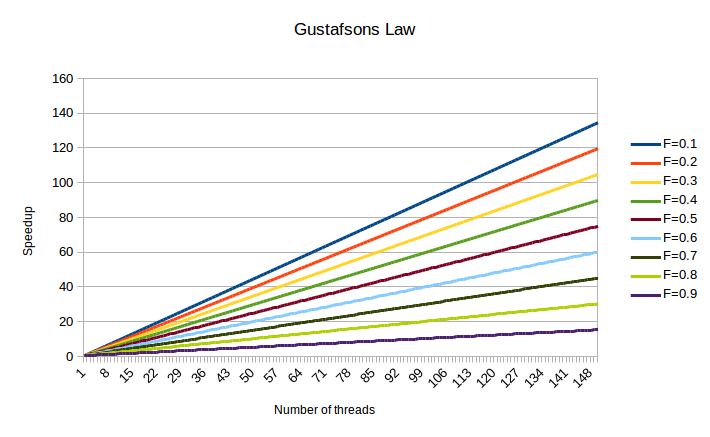
\includegraphics[width=13cm]{GustafsonsLaw.png}
    \caption{Illustration of Gustafsons Law}
    \label{fig:GustafsonsLaw}
\end{figure}

\subsubsection{Profilers}
There are applications called profilers that are made to assess the programs performance and resource consumption. They calculate some of the measures mentioned earlier and they also check hardware usage and how much time the program spends at various parts of the program. This is very useful for finding bottlenecks and other problems in the program. It does not matter if the algorithm is super fast if all the data is stuck in network transfers. The profilers can be hardware dependent so the manufactures usually provided them for their products. For instance NVIDIA provides profilers for programs that use CUDA.\cite{introduction_hpc_hager, cuda_best_practice}

\clearpage
\section{Software Design}
How to design software so it can be mainted over time .

The messier code will cost productivity in the future when bugs and other problems stack up because of earlier misstakes. All code aquire problems overtime however a well designed system will degenerate a lot slower than one that was designed without much thought. Our code will also be read by others and ourselves later which means readability is important.

%study om repro in comp science
%anv�nde repeabtibility ist�llet f�r reproducebility

There are ways to code in such a way that these problems can be avoided. Most of the things described here goes under the agile development type and the concept of clean code. SOLID is an acronym for five principles for object oriented programming and design. When used together they are intended to make programs that are easy to maintain and extend. One of the first things to keep in mind that others and ones future self will likely read the code. This means that it has to be written so that things are as clear as possible. Correct names will make the code explain itself without other documentation, the code itself is the documentation.

\begin{table}[h]
\begin{tabular}{ l l l}
  \hline
  Initial & Principal & Concept\\
  \hline
  S & Single responsibility principle & A class should only have a single responsibility \\
  O & Open/closed principle & A class should be open for extension but closed for modification \\
  L & Liskov substitution principle & If S is a subtype of T, then objects of type T may be replaced by objects of type S without without altering any of the desierable properties of the program(e.g. work performed)\\
  I & Interface segregation principle & Use several smaller and more specific interfaces instead of one large \\
  D & Dependency inversion principle & Depend on abstractions(e.g. interfaces) not details \\
  \hline  
\end{tabular}
\caption{The five SOLID principles}
\label{table:solid_table}
\end{table}

Dependacy injection is one way to implement dependacy inversion principle. Injection is passing the dependacy to the dependent object. This is used instead of allowing the depedent object to construct or find the dependacy.

\subsection{Unit Tests and Mocks}
\emph{Unit testing} involves testing the program in small units in isolation. Testing in isolation means that the test should only depend on the part of the program that is tested. If a part of the program is not working properly only its related tests should fail, not other tests for code that depends on it but otherwise works properly. This makes it easier to find errors when they do occur since the tests will pinpoint the unit which does not work.\\
\\
It is easy to denote test code as less important than the main code but they should be treated as equally important. Tests should also not be an incovieance to use so they should be easy to run, take reasonable ammount of time to complete and not require any outside interpretation whtever they failed or not.\\
\\
\emph{Mocking} is to replace a real object with a fake object called a \emph{mock} that for the code is indistinguishable from the real object. This allows one to create situations and test with more control and without depending on the real objects code. The second is important for unit tests since it enables one to test units that normally depend on others in isolation. In the first case it is useful in situatuons such as when one wants to test a class handling of a rare failure. Such failures can be hard and time consuming to induce. It is then easier to use a mock object that behaves like the failure has accured. However mocking requires that the code for the class doesn't create the object itself since there is no way to replace the object with the mock. This is one of the reasons why dependacy injection should be use.

\subsection{Design Patterns}
A \emph{design pattern} in software design is a reusable general solution to a common reacurring problem in a given context. It is templates and structures to solve the problem, however it is not code. However they are partially dependent on the programming language since different langauages have different features and limitations.\\
\\
The \emph{? pattern} %example pattern?
\\
\emph{Concurrancy patterns} are design patterns in contexts which involves concurrancy, i.e. multithreaded programs.

locks

\emph{Consumer producer} is a pattern for when there are a number of consumers/workers and producers. They share a common queue for products. The producer generates some product and put it into the queue, while the the consumers consume the products. The problem is that the producers should not add to an non empty slot and that each product should only be consumed once.

%cite http://www.objectmentor.com/resources/articles/Principles_and_Patterns.pdf
%cite clean code

\clearpage
\chapter{Algorithm}
%Algorithm (up till 20 pages)
%  - Current state - Basic algorithm, Data structure, memory consumption, parallelization, load balancing and scalability
%  - And the same for own your implementation

%TODO nån typ av intro här

%OTHERS
%problem with exathsutive

%memory problems(GENIE, CUDALR and so on)

%2 bit 3 bit data storage

%two stage analysis


\section{Current algorithm}
JEIRA uses Java and Javas built-in functions for concurrency.

Producer consumer pattern

%strucuture picture

\section{CuEira}
%exhaustive

Producer consumer pattern ?

Strucuture picture here.

%optimizations
unrolling+padding
compilers

\chapter{Results}
%Results (up till 15 pages including plots)
%  - Performance measurements (scalability, speed up and efficiency as well as load balancing)
%  - Setup(simulation setup, compilers and hardware setup)
%  - Single node performance
%  - multy-node performance


%What was used
%Zorn specs
%compiler intel 13.1
%cmake 2.8
%mkl 13.1
%cuda 5.5

\chapter{Discussion and Conclusions}
%Discussion and Conclusions (up to 3 pages)
%Need for novel methods for gene-environment interaction
%Need for methods for third order interaction and higher

\chapter{Outlook}
%Outlook (up to one page)

cublas not that much harder than regular blas. A wrapper could enable simple and easy use without losing too much features.
own kernels more than simple elemntwise, probably hard to optimize. unknowish

\chapter{Appendix}
\section{A List of Variables}

\begin{description}
%anything with hat is estimate
\item[OR]
  Odds ratio
\item[$RR_{ij}$]
  Relative risk with exposure i j?
\item[X]
  Predictors
\item[Y]
  The outcome, binary variable
\item[$\pi(x)$]
  P(Y=1)
\end{description}

\section{B List of Abbrivations}

\begin{description}
\item[MAF] \hfill \\
  Minor allele frequency, the frequency of the least common allele.
\item[RF] \hfill \\
  Random Forest
\end{description}

%List of figs
%List of tables


\newpage
\bibliographystyle{ieeetr}
\bibliography{hpc.bib,statistics.bib,misc.bib}
\end{document}